
%(BEGIN_QUESTION)
% Copyright 2012, Tony R. Kuphaldt, released under the Creative Commons Attribution License (v 1.0)
% This means you may do almost anything with this work of mine, so long as you give me proper credit

Machinists use a tool called {\it calipers} to measure short distances such as the outside diameter of a shaft.  One particular type of caliper has a special scale that slides along with the movable jaw called a {\it vernier} scale.  The spacing between divisions on the vernier scale is slightly less than the spacing between divisions on the main scale, which means only one division on the vernier scale will ever line up with a division on the main scale at any given time:

In order to obtain a coarse measurement of the caliper's jow position, read the main scale using the ``0'' mark on the vernier scale as a pointer:

$$\includegraphics[width=15.5cm]{i01128x01.eps}$$

\filbreak

Now, use the vernier scale to read the distance between the caliper's jaws, when the ``0'' division on the vernier scale does {\it not} line up perfectly with one of the divisions on the main scale:

$$\includegraphics[width=15.5cm]{i01128x02.eps}$$

\underbar{file i01128}
%(END_QUESTION)





%(BEGIN_ANSWER)

Distance = 0.93
 
%(END_ANSWER)





%(BEGIN_NOTES)


%INDEX% Mechanics, reading an analog scale (vernier)

%(END_NOTES)


